\chapter{L'Architechture CORBA}

    \section{Qu'est ce que le cadre CORBA ?}

        \par CORBA est l’acronyme de \textit{\textbf{C}ommon \textbf{O}bject \textbf{R}equest \textbf{B}roker \textbf{A}rchitecture}. Il s’agit d’un standard développé en 1992 par Object Management Group (ou OMG) ; un consortium de plusieurs centaines d’entreprises dédiées à la construction de matériel informatique et l’édition de logiciels.\\
        L’objectif est de développer des applications distribuées indépendantes de la plate-forme et du langage à travers des principes de conception orientés objet.\\

        Corba repose sur la notion de bus logiciel (Object Request Broker).
        En Corba, tout est objet. On bénéficie donc des mécanismes d'héritage, polymorphisme et encapsulation.

    \section{Les avantages de Corba}

        \begin{itemize}[label= \ding{51}]
            \item \textbf{Interopérabilité: }Les objets Corba communiquent par l'intermédiaire du protocole IIOP (Internet Inter-ORB Protocol). Ce protocole permet la communication entre entités quelconques supportant le protocole TCP/IP.
            \item \textbf{Intégration aux systèmes existants: }Tout code existant peut être encapsulé dans un objet Corba (wrapping). Des passerelles existent pour des standards de distribution d'objets du marché (DCOM, DCE).
            \item \textbf{flexibilité du développement: }Les services rendus par les objets sont définis par leur interface qui tient lieu de contrat entre l'utilisateur et le fournisseur du service. Les parties définition et implantation d'un objet sont totalement dissociées.
        \end{itemize}

    \section{Objets distribués de CORBA}

        \begin{itemize}
            \item  Localisation indifférente dans le réseau;
            \item Sur des systèmes hétérogènes;
            \item Implantés dans des langages différents.
        \end{itemize}
\pagebreak
    
    \section{Composants logiciels}

        \begin{itemize}
            \item  Accédés par n'importe quel client;
            \item Via des invocations de méthodes;
            \item Le client ne connait que l'interface publiée par le serveur;
            \item L'interface est spécifiée dans un langage standard l'IDL.
        \end{itemize}

    \section{Le modèle objet client-serveur CORBA}

    Il est fondé sur une entité virtuelle, l'objet CORBA, gérée par le bus CORBA. Chaque application peut exporter ses services sous la forme d'objets CORBA.
    La coopération client-serveur se déroule de la manière suivante :
    \begin{enumerate}
        \item  Le client détient une référence sur un objet CORBA qui permet de le localiser sur le bus.
        \item Le client dispose de l'interface de l'objet CORBA (type abstrait de l'objet CORBA) qui définit ses opérations et ses attributs (exprimés dans le langage IDL).
        \item Le client réalise une requête (invoque) une opération sur l'objet CORBA.
        \item Le bus CORBA achemine cette requête vers l'objet CORBA tout en masquant les problèmes d'hétérogénéité liés aux langages, systèmes d'exploitation, machines, réseaux.
        \item L'objet CORBA est associé à un objet d'implantation
        \item Le serveur détient l'objet d'implantation qui code l'objet CORBA (cette implantation pouvant évoluer au cours du temps) et gère son état temporaire.
    \end{enumerate}
    \vfill

    \begin{figure}[h]
        \centering
        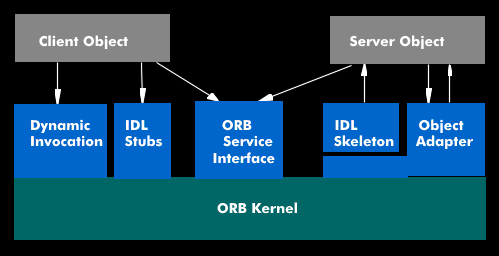
\includegraphics[scale= 0.77]{archiCorba/CORBA-Architektur.png}
        \caption{CORBA Architechtur}
    \end{figure}

        


    
    